\documentclass{scrartcl}

\usepackage[utf8]{inputenc}
\usepackage[T1]{fontenc}
\usepackage{lmodern}
\usepackage[english]{babel}
\usepackage{amsmath}
\usepackage{graphicx}
\usepackage{caption}	
\usepackage{subcaption}	 
\usepackage{hyperref}
\usepackage[parfill]{parskip}
\usepackage{hhline}
\usepackage{subcaption}

\title{Neuroprosthetics - Exercise 3}
\author{Alexander Koenig}
\date{30. November 2019}

\begin{document}
\maketitle

\section{Solver Implementation}

An initial value problem (IVP) $\frac{dV}{dt} = f(V,t)$ with a given $V(t_0) = V_0$ may be solved numerically using a variety of methods. The following numerical solvers for differential equations were implemented in Python. Starting from a given initial value $V_0$ the next value $V_{n+1}$ can be calculated using the following formulae.

\textbf{Explicit Euler Method}
\begin{equation}
	\label{eq:explicit_euler}
	V_{n+1} = V_n + f(V_n, t_n)\cdot \Delta t
\end{equation}

\textbf{Heun's Method}
\begin{align}	
	\label{eq:heun}
	&A = f(V_n, t_n) \\
	&B = f(V_n + A \cdot \Delta t, t_{n+1}) \\
	&V_{n+1} = V_n + \frac{A + B}{2} \cdot \Delta t
\end{align}

Equations of the form $\frac{dV}{dt} = A(t)V(t) + B(V,t)$ may be solved with exponential methods such as the Exponential Euler Method.

\textbf{Exponential Euler Method}
\begin{equation}
	\label{eq:exponential_euler}
	V_{n+1} = V_n e^{A(t_n) \cdot \Delta t} + \frac{B(V_n,t_n)}{A(t_n)}(e^{A(t_n) \cdot \Delta t} - 1)
\end{equation}

\newpage
\section{Solve Functions}

The initial value problem in equation \ref{eq:ivp} is solved with the above methods in the interval $t \in [-4.5s, 5s]$ with varying step sizes. It becomes obvious from the plots (figure \ref{fig:explicit_euler}, \ref{fig:heun} and \ref{fig:exponential_euler}) that reducing the step size of the respective numerical integration scheme from $1s$ to $0.012s$ yields a more accurate result. However, smaller step sizes come at a computational cost, as more calculations have to be executed. Therefore using an infinitesimal step size is not computationally feasible.

\begin{align}
	\label{eq:ivp}
	&\frac{dV}{dt} = 1- V - t \\
		&V(t=-4.5) = V_0 = -4 \nonumber
\end{align}

\begin{figure}[h]
	\centering
	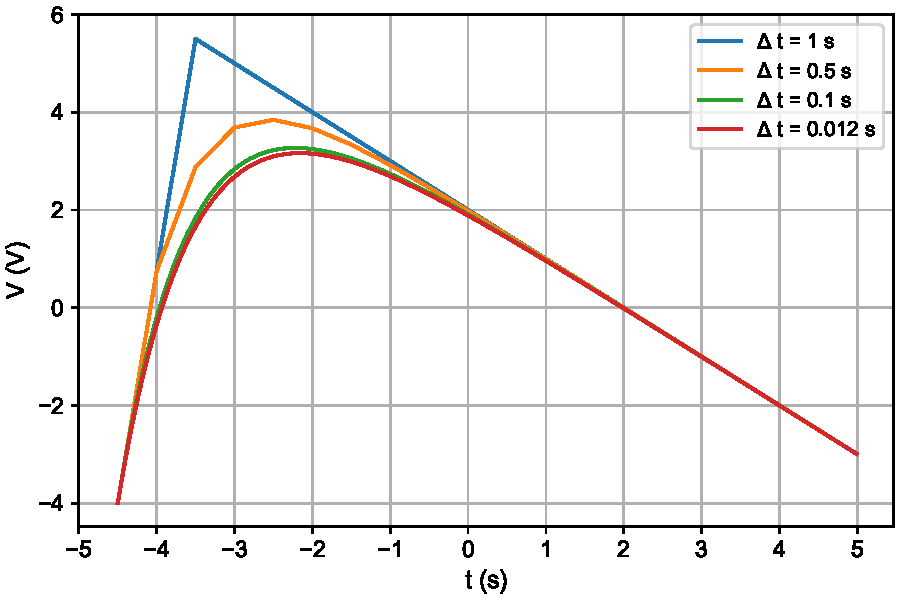
\includegraphics[width=0.9\textwidth]{figures/explicit_euler.pdf}
	\caption{Numerical solution using Explicit Euler}
	\label{fig:explicit_euler}
\end{figure}
\begin{figure}[h!]
	\centering
	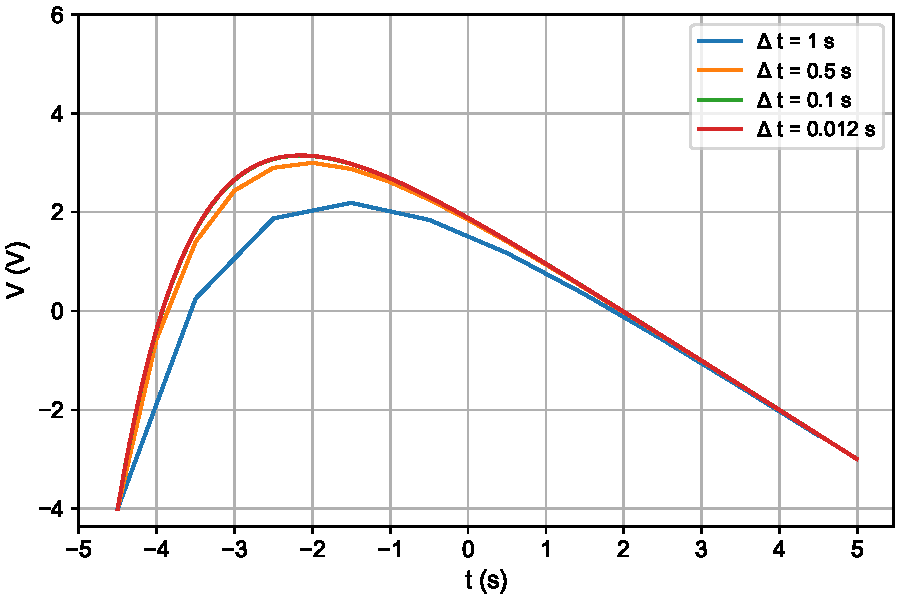
\includegraphics[width=0.9\textwidth]{figures/heun.pdf}
	\caption{Numerical solution using Heun}
	\label{fig:heun}
\end{figure}
\begin{figure}[h!]
	\centering
	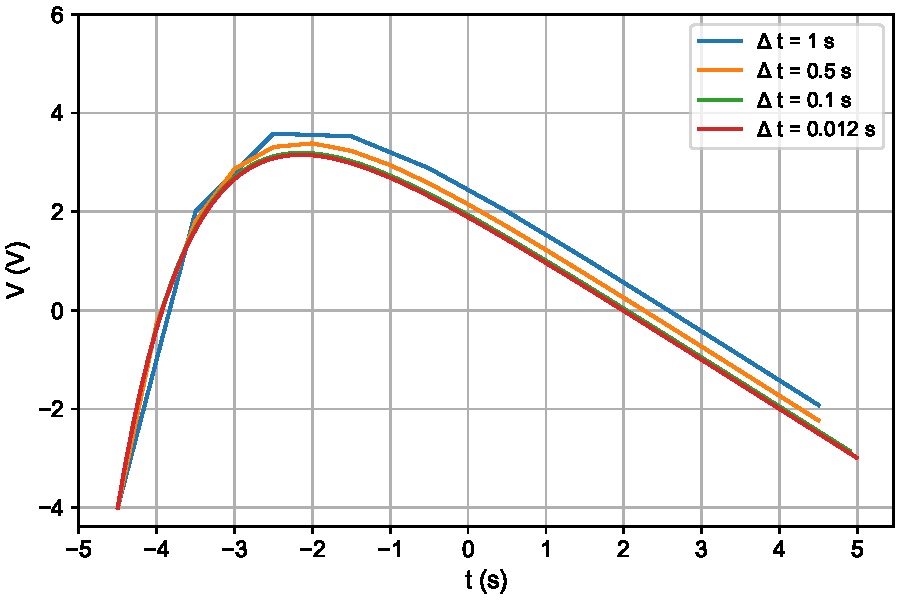
\includegraphics[width=0.9\textwidth]{figures/exponential_euler.pdf}
	\caption{Numerical solution using Exponential Euler}
	\label{fig:exponential_euler}
\end{figure}

\newpage
\section{The Leaky Integrate and Fire Neuron}

The cell membrane voltage of the Leaky Integrate and Fire (LIF) Neuron can be modeled with equation \ref{eq:lif}. In this example, the external current $I_{ex}$ that stimulates the neuron is either modeled as a constant current ($10\mu A$ and $20\mu A$) or a rectified sine wave (50Hz with $10\mu A$ and $20\mu A$ amplitude). The rectified sine waves are displayed in figure \ref{fig:sine}. 

\begin{equation}
\label{eq:lif}
V_{n+1}=\left\{\begin{array}{ll}{V_{n}+\frac{\Delta t}{C_{m}}\left(-g_{l e a k}\left(V_{n}-V_{r e s t}\right)+I_{ex}\left(t_{n}\right)\right)} & {V_{n}<V_{t h r}} \\ {V_{s p i k e}} & {V_{t h r} \leq V_{n}<V_{s p i k e}} \\ {V_{r e s t}} & {V_{s p i k e} \leq V_{n}}\end{array}\right.
\end{equation}

with 
\vspace{0.2cm}
\begin{itemize}
	\item $V_n$: cell membrane voltage
	\item $C_m = 1\mu F$: membrane capacitance
	\item $g_{leak} = 100\mu S$: leak conductivity
	\item $V_{rest} = -60mV$: cell membrane resting voltage
	\item $V_{thr} = -20mV$: cell membrane spiking threshold voltage
	\item $V_{spike} = 20mV$: spiking voltage
\end{itemize}


\vspace{0.7cm}
The model in equation \ref{eq:lif} describes the process of charging and discharging a capacitor with an input current through a resistor. When a constant current is applied to the neuron (see figure \ref{fig:V_const}) the cell membrane voltage of the LIF neuron exponentially increases until a certain threshold voltage is reached. When the threshold is reached the voltage spikes and an action potential occurs. After the spike, the transmembrane potential reaches the resting potential and the process is repeated at a constant rate. Notably, the constant input current is directly proportional to the frequency of charge and discharge cycles.

For the rectified sine input current the process is very similar in that there is still a repeated cycle of charge and discharge of the capacitor (see figure \ref{fig:V_sine}). The main difference is that the charging process of the capacitor now follows a different profile. In some cases, the charge from the capacitor can flow back before the threshold is reached and hence a curved transmembrane potential can be observed in these time intervals. Further the rate at which the neuron fires is not constant for the rectified sine input current. 

\begin{figure}[p]
	\centering
	\begin{subfigure}{\textwidth}
	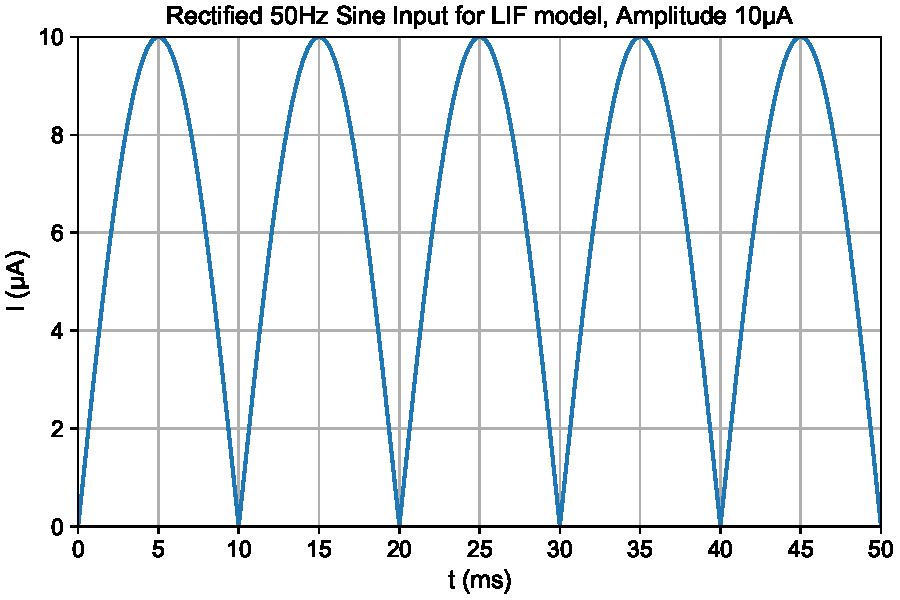
\includegraphics[width=0.9\textwidth]{figures/sine_10.pdf}
	\vspace{0.8cm}
	\end{subfigure}
	\begin{subfigure}{\textwidth}
	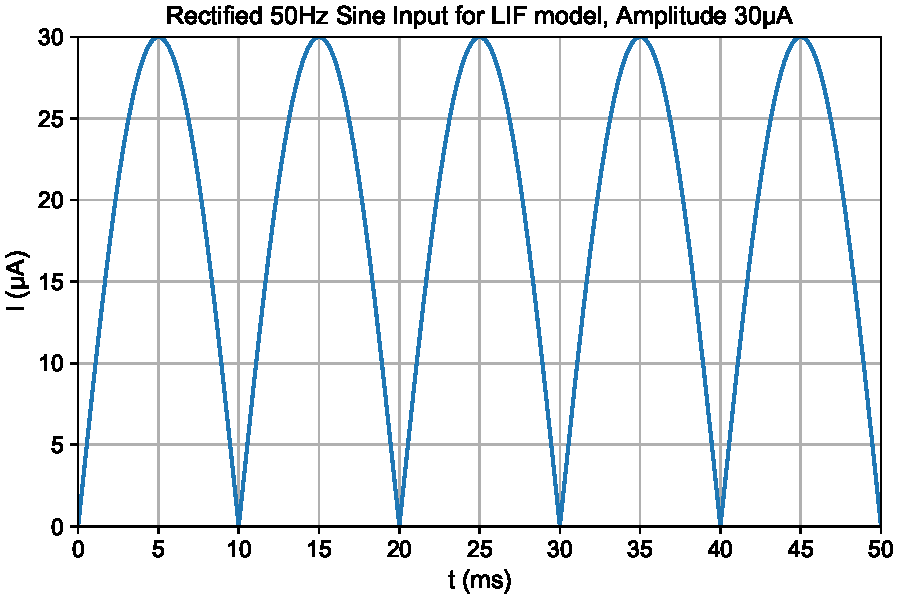
\includegraphics[width=0.9\textwidth]{figures/sine_30.pdf}
	\end{subfigure}
	\vspace{0.8cm}
	\caption{Input currents}
	\label{fig:sine}
\end{figure}

\begin{figure}[p]
	\centering
	\begin{subfigure}{\textwidth}
	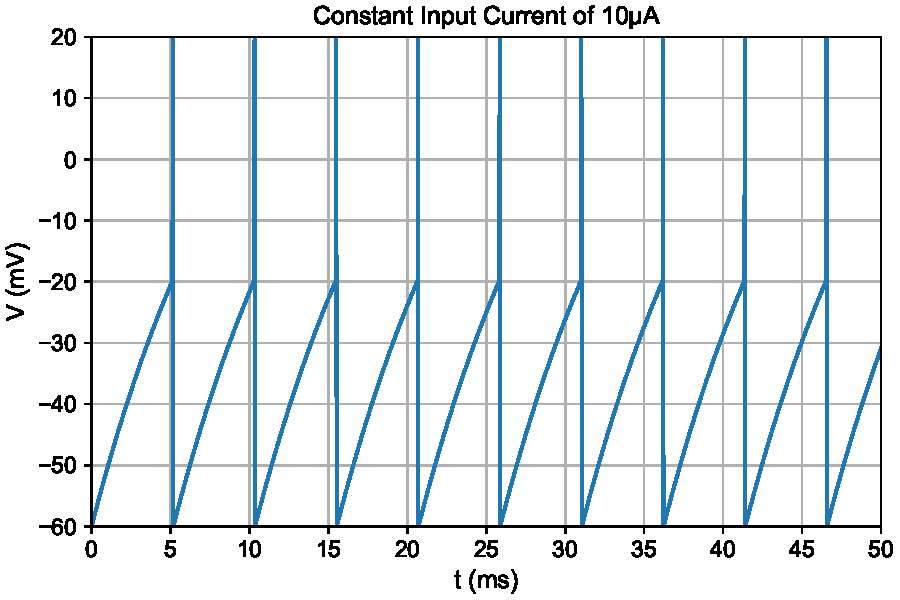
\includegraphics[width=0.9\textwidth]{figures/V_const_10.pdf}
	\vspace{0.8cm}
	\end{subfigure}
	\begin{subfigure}{\textwidth}
	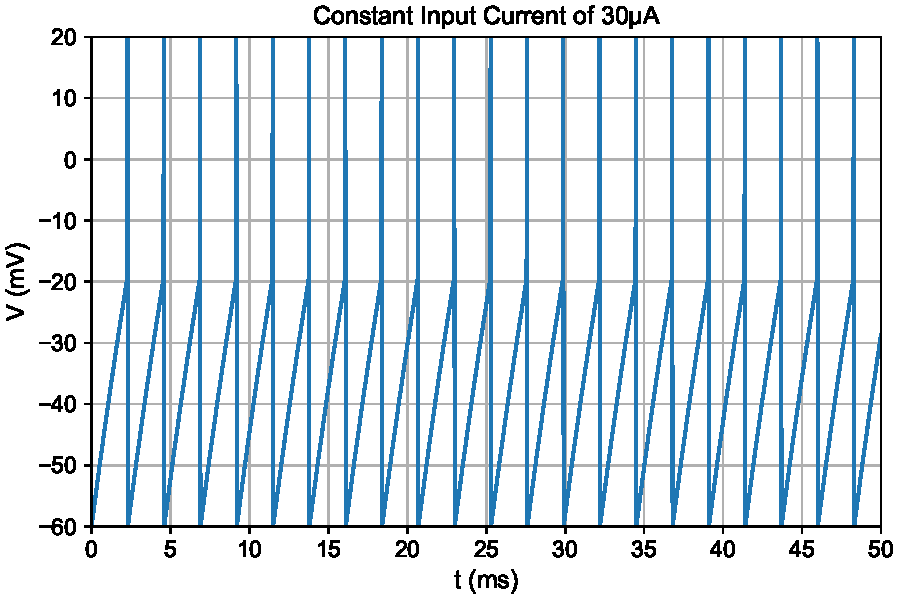
\includegraphics[width=0.9\textwidth]{figures/V_const_30.pdf}
	\end{subfigure}
	\vspace{0.8cm}
	\caption{Membrane voltage with constant input current}
	\label{fig:V_const}
\end{figure}

\begin{figure}[p]
	\centering
	\begin{subfigure}{\textwidth}
	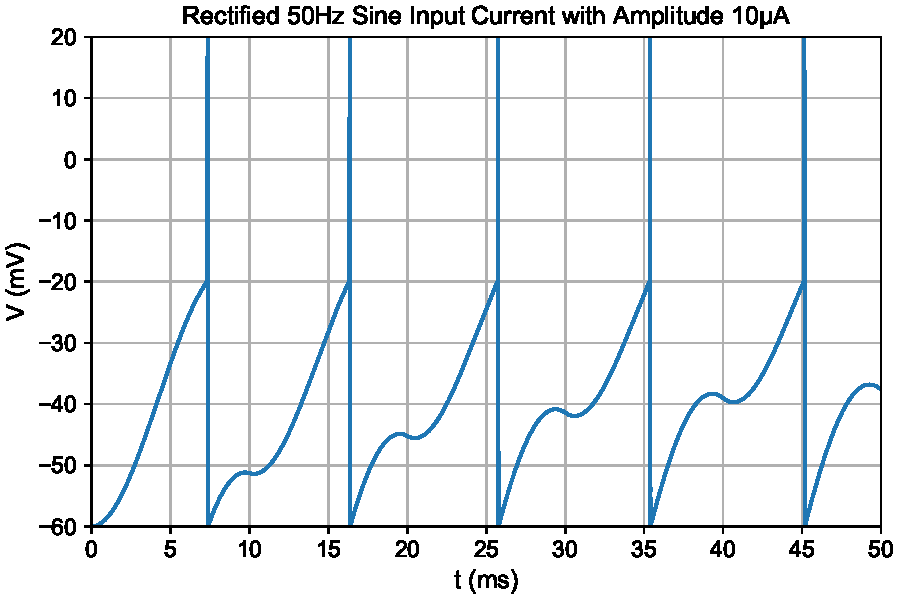
\includegraphics[width=0.9\textwidth]{figures/V_sine_10.pdf}
	\vspace{0.8cm}
	\end{subfigure}
	\begin{subfigure}{\textwidth}
	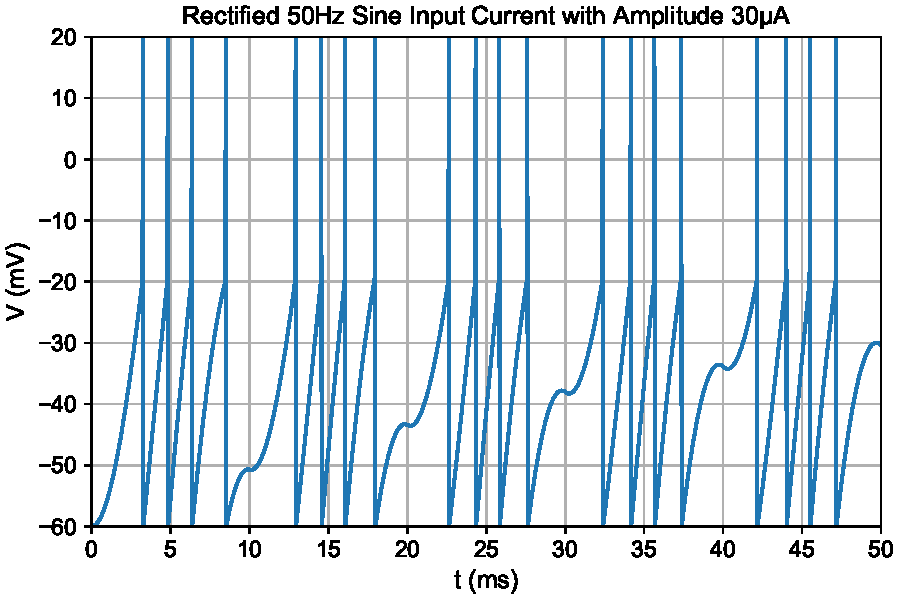
\includegraphics[width=0.9\textwidth]{figures/V_sine_30.pdf}
	\end{subfigure}
	\vspace{0.8cm}
	\caption{Membrane voltage with rectified sine input current}
	\label{fig:V_sine}
\end{figure}


\end{document}